\chapter{Methodology}
    \label{chap:methodology}
    
\section{Research methodology}

The research hypothesis of this project is the following: 

\textit{It is possible to use a generative neural network to create 3D-rendered adversarial objects in the targeted black-box setting that have a targeted fooling rate of at least 50\% on a victim CNN classifier for object recognition.}

\bigbreak
3D-rendered adversarial objects were described in subsection \ref{subsubsec:eot}. The targeted fooling rate metric is explained in subsection \ref{sec:analytic_techniques}. The 50\% threshold is chosen because an attack can be considered effective if it is more likely to succeed than fail.

I believe that the hypothesis is true because the black-box generative model in subsection \ref{subsubsec:zheng} can be easily combined with the EOT framework for making adversarial objects in subsection \ref{subsubsec:eot}. I think this is feasible because EOT virtually augments the dataset with images of an object in various poses so that the adversarial perturbation is robust \cite{athalye}. The same thing can be done with the perturbations generated by the generator described in subsection \ref{subsubsec:eot} before they are sent to the simulator.

Moreover, I plan to use generative models for creating black-box adversarial perturbations rather than other methods as they have proven to have high fooling rates \cite{upset_angri, zheng_black_box_GAN}.

This is an experimental research project. The model proposed in subsection \ref{subsubsec:architecture_design} will create 3D-rendered objects, and pictures of those objects will be given to various neural network classifiers. The predicted label will be compared against the correct label and the adversarial target label to evaluate the effectiveness of the proposed method. Further details on the experiments are found in subsection \ref{sec:experiment_design}.

\section{Architecture design of GAN-EOT}
    \label{sec:architecture_design}
    
The proposed GAN-EOT is almost the same generative model presented in subsection \ref{subsubsec:zheng}, except that it has elements of the EOT framework \cite{athalye} added to it. The key difference is that the generator produces adversarial perturbations for a 2D texture rather than an image of an object, as you can see in figure \ref{fig:proposed_model}. Moreover, the adversarial texture is then rendered as a 3D object, and an image of the rendered object is then given to the simulator.

\begin{figure}[h]
    \centering
    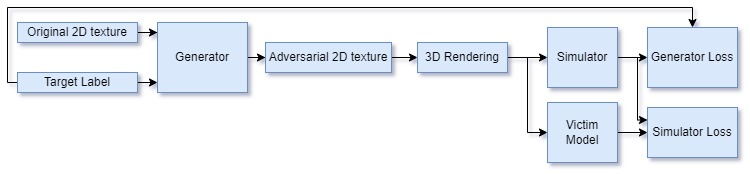
\includegraphics[width=1\textwidth]{graphics/model.jpg}
    \caption{The architecture of the proposed generative model.}
    \label{fig:proposed_model}
\end{figure}

The 3D rendering will simulate a variety of transformations such as 3D rotation, translation, varying camera distance, different background and lighting conditions, and 3D printer errors, just like it was done in the EOT framework from subsection \ref{subsubsec:eot}. I will be using the same distribution $T$ of transformation functions as \cite{athalye} did, though perhaps with different bounds for the uniform distributions. The mini-batches used at each training step shall be constructed as described in the penultimate paragraph of subsection \ref{subsubsec:eot}.

The generator will have the same structure as the one in figure \ref{fig:generator} in subsection \ref{subsubsec:zheng}. The simulator will again be a CNN, and I will experiment with the 4 simulator architectures used in \cite{zheng_black_box_GAN}, though other CNNs might be included as well. Moreover, the simulator will be trained in the same way as subsection \ref{subsubsec:zheng} describes. The generator will also be trained as equation \ref{eq:generator_loss} on page \pageref{eq:generator_loss} describes, except that the penalty term will be replaced by:

\begin{equation}
    \begin{aligned}
    \beta\|LAB(t(x + G(x,z))) - LAB(t(x))\|_2
    \end{aligned}
\end{equation}

\noindent because the $LAB$ space distance metric encourages imperceptibility to the human eye.

I chose to use EOT \cite{athalye} rather than $\textrm{RP}_2$ \cite{evtimov_road_signs} because it is a lot more convenient. $\textrm{RP}_2$ requires the user to manually take a lot of photos and to manually create the perturbation mask $M_x$. Furthermore, the authors of \cite{evtimov_road_signs} do not offer any detailed information on how the perturbation alignment function $T_i$ works, not even in the supplementary material. Finally, their approach is only applicable to flat physical surfaces, like road signs. On the other hand, EOT works for any 3D object \cite{athalye}, and could also use a mask to create adversarial patches like \cite{evtimov_road_signs} did. Finally, the synthetic transformation functions for 3D rendered objects can accurately simulate real-world transformations \cite{athalye}.

Regarding the 3D renderer, it must be able to take a 2D texture and render it as a 3D object. It must support 3D rotation, translation, perspective projection, different background colours, and additive and multiplicative lighting. Moreover, since the transformation functions $t(\cdot)$ simulate 3D rendering and must be differentiable, the chosen renderer must return the texture-space coordinates. Athalye \textit{et al.} \cite{athalye} do not say which specific renderer they used, they just modified an existing renderer to return that information. Therefore, this project will do the same.

\section{Analytic techniques}
    \label{sec:analytic_techniques}
    
Unless otherwise specified, each experiment will use both of the following metrics to evaluate the proposed attack's success:

\begin{itemize}
    \item \textbf{Targeted Fool Rate (TFR):} the percentage of adversarial examples that are classified by the victim model as the desired target label.
    \item \textbf{Untargeted Fool Rate (UFR):} the percentage of adversarial examples that are classified by the victim model as any incorrect label. It is relevant because if the attack induces a misclassification, even if it is not the desired target label, then it is still dangerous.
\end{itemize}

The authors of \cite{zheng_black_box_GAN} use these metrics but do not say whether they only consider adversarial examples whose original image is correctly classified. In my experiments, I will only consider the latter, because if the original image is already misclassified by the victim model, then the effect of the adversarial example is meaningless.
